\documentclass[journal]{IEEEtran}
% *** CITATION PACKAGES ***
\usepackage{cite}
\usepackage{graphicx}
%\usepackage[style=numeric-comp]{biblatex}
% *** GRAPHICS RELATED PACKAGES ***

% graphs with tikz
\usepackage{pgfplots,pgfplotstable}
\usepackage{tikz}
\usetikzlibrary{arrows,positioning,fit,backgrounds} 

\hyphenation{op-tical net-works semi-conduc-tor}

%%% TODO marks
\usepackage{color}
\newcommand{\todo}[1]{

    \textcolor{red}{\hspace{-2cm} TODO: #1}
    \PackageWarning{TODO:}{#1!}
}


\begin{document}

\title{Smart File System}

\author{Fabian Spie\ss, Max Mustermann}
        
% make the title area
\maketitle


\begin{abstract}
%\boldmath
The abstract goes here.
\end{abstract}

\IEEEpeerreviewmaketitle

\tableofcontents


\section{Introduction}
\IEEEPARstart{T}{his} demo file is intended to serve as a ``starter file''
for IEEE journal papers produced under \LaTeX\ using
IEEEtran.cls version 1.7 and later.
I wish you the best of success.

\hfill mds
 
\hfill January 11, 2007

\section{The Systemarchitecture}


\IEEEPARstart{B}{ased} on project restrictions and own decisions there was a hardware and software mixed test system created. This chapter will give a short introduction about how all the system parts are connected to each other. Detailed description about single parts will follow later.

\subsection{Hardware Setup}

Given by the project initiator, the institute for complex and distributed IT systems of TU Berlin (CIT) some hardware components were directly defined as prerequisites.

\begin{enumerate}

\item One powerful machine placed in tubit data centre (TU Berlin), later called by it's name \textit{Asok05}.

\item One energy-saving \textit{office pc} attached to TU network inside a staff office with lower bandwidth.

\item Two energy meters called \textit{EGM-PWM-LAN} of the brand \textit{Energenie} which were used to measure the power usage of \textit{Asok05} and the \textit{office pc}.

\item To run services which should not influence the power usage measured by the energy meters, a virtual machine, placed in the tubit data centre was prepared to be used too.

\end{enumerate}

\todo{add some machine details (storage/bandwidth/power/power usage idle)}

\subsection{Software Setup}

The introduced and following software systems were used by own decisions described later.

\begin{enumerate}

\item As distributed file system which controls the filesystem access the Apache Haddop\textsuperscript{\textregistered} Filesystem (HDFS) was used, described in chapter~\ref{sec:dfs}. The access to filesystem may be done using a terminal, http or a client as provided by Filesystem in Userspace (FUSE), a web client or terminal window. HDFS consists of two main parts, the namenode which organises the filesystem structural view, and datanodes which organise the stored amount of data in blocks.

\item To measure network traffic, all data were sent through a virtual network. A combination of Floodlight as controller and an Open vSwitch was used, described in chapter~\ref{sec:sdn}. 

\item For monitoring user actions in the filesystem and on the network we have used a zabbix server. this service collects data sent by an zabbix agent. \todo{chapter ref}

\item To analyze the changes in energy consumption produced by user activities the energy consumption of \textit{office pc} and \textit{Asok05} were measured. \todo{chapter ref?}

\item By evaluating the monitored data we were able to create a  report which informs about the power consumption used by all or a specified user. \todo{chapter ref}

\end{enumerate}

\subsection{Services Setup}

The distribution of services used in project are given in table~\ref{tab:services}.

\begin{table}[b]
	\centering
	\caption{Services and machines overview used in project. }
	\begin{tabular}{|l|l|l|l|l|}
		\hline \rule[-2ex]{0pt}{5.5ex} \textbf{client pc} & \textbf{office pc} & \textbf{virtual machine} & \textbf{Asok05} \\ 
		\hline \rule[-2ex]{0pt}{5.5ex} hadoop client & hadoop data node & hadoop name node & hadoop data node \\ 
		       \rule[-2ex]{0pt}{5.5ex}  & energy meter & zabbix server & energy meter \\ 
		       \rule[-2ex]{0pt}{5.5ex}  & zabbix agent & zabbix agent & zabbix agent \\ 
		       \rule[-2ex]{0pt}{5.5ex}  &  &  & Floodlight \\ 
		       \rule[-2ex]{0pt}{5.5ex}  &  &  & Open vSwitch \\ 
		       \rule[-2ex]{0pt}{5.5ex}  &  &  & energy data agent \\ 
		\hline 
	\end{tabular}
	\label{tab:services}
\end{table}


\section{Filesystem}
\subsection{From local to distributed filesystems}

\todo{which word to use? distributed filesystem (dfs)?}
\todo{maybe duplicates the introduction}
\todo{is it clear that a san keeps storage for one machine and a dfs shares storage for different users/machines better?}

To offer multiple users and applications a high available access on large filesystems there are different solutions known. 
Files can be stored on local filesystems, or may be shared using a network attached storage (NAS) for small businesses or for use at home. 
While a local filesystem is strongly limited to capacity and multi user access a NAS allows to have an system available for different users. 
But a NAS is limited for a small number of users and very much limited in world wide file sharing and a secure 24h availability.

A first solution to offer data stores for multiple machines which is actually common in data centers is to setup a storage area network. 
This system may store different filesystems for different client machines without being limited to the speed of one pysical harddrive. 
For security reasons it is possible to keep a redundant copy of such a system in a different place and exporting backups too. 
But is is not quite easy to resize that system and not the best solution for sharing same view of the data to different machines and machines placed outside of a data centre.

Companies like Facebook were facing these issues and solved them using a distributed filesystem (DFS) \cite{fb-hadoop}. 
The use of an DFS allows to raise the cluster storage  up to petabytes  \cite{fb-hadoop}. 
A lot of huge different companies already have decided, to use hadoop to store and backup their data  \cite{hadoop-poweredby}. 
Different algorithms such MapReduce are used to share limitations of cpu power and storage between clustered nodes \cite{dean2008mapreduce}. 
Further it is easy to raise the number of nodes which makes it highly flexible to use. Only the power in administration will raise, cyaused on the number of heterogeneus machines, too.

For cases such as downloading huge files as operating system images it is important to find strategies for reducing traffic by only updating changed parts of such files, named random write.
Different interesting questions are about creating snapshots or creating and applying backups where google was focusing on for their own filesystem implementation \cite{ghemawat2003google}.

Similar functionalities are available through the replacement of FibreChannel by iSCSI for SAN. But the use of such a system will limit to one manufacturer. Maybe thats one of the main reasons which makes distributed filesystems so popular.

\subsection{Introduction of Apache Hadoop}

The distributed filesystem (DFS) should be used to connect cloud storage with a client machine as being local storage as shown in figure~\ref{fig:dfs_example}. To mount the network storage as being local a client program has to be running on the client machine. By using the DFS it will remove local limitations on Storage while offering a given QoS for bandwidth and multiuser support.

\todo{create a simplified copy in a better fitting style}

\begin{figure}
	\centering
	\includegraphics[width=1\linewidth]{img/dfs_example.png}
	\caption{Basic idea of mounting a distributed filesystem}
	\label{fig:dfs_example}
\end{figure}

A research of known DFS brought us the choice between GlusterFS and Apache Hadoop.

GlusterFS is developt by Red Hat inc. and written in C. Hadoop is part of Apache and written in Java.

Both are open souce and can be easily extened by our own plugins. In addition, both offers a very active community and therefore a steady development. The support of Java was the main reason for hadoop. So our decision was made.

\todo{move client information to this chapter???}

\subsection{Hadoop setup}

By creating a small cluster in the tubit data centre the power consumtion that is used for the system itself and by performing user actions like up- and downloading files is analyzed.

For our test system we have used the distributed filesystem (DFS) Apache Hadoop\textsuperscript{\textregistered}. This system was used due to the idea having an DFS running on heterogeneus systems from different hardware and operating systems based on Java. 

Hadoop consits of two main parts. A nameserver that keeps the logic view of the filesystem and a various number of datanodes which keep the files organized in blocks of a fixed length. Multiple datanodes can be used to raise the available storage amount or to keep multiple replicas of files in different locations for security reasons or to share power between different machines. 

The datanodes were placed on the physical machines of our test system, \textit{Asok05} and the \textit{office pc}. Both are different in power consumption and maximum of provided bandwidth. A connection to the namenode which is placed on the virtual machine was made through a software defined network which is described in chapter\ref{sec:sdn}.

To assign network traffic to users different attributes were sent to zabbix like client username, client ip and port on requests to a modified datanode.
Combined with the information of software defined network it was possible to get an overview of current user bandwidth. Further the traffic amount for a time range was calculated. The namenode was used for sending the current user storage amount to the monitoring system.

\subsection{Data delivery strategies}

The namenode is responsible to establish the first client connection. By recieving a file download request it will respond with a list of file blocks, and the assigned datanode locations. By varying the block list, different power consumption optimizations were analyzed.

After recieving the list of data blocks and related locations, the client application decides which locations for each data block should be chosen as download location. After that step the client application creates the file as local copy from all downloaded data blocks by itself. By reducing the block locations list before sending to the client we commanded which locations should be used from the client application.

\subsubsection{server selection for downloading files}

By comparing the power consumption while downloading files and while being idle the following values were measured.

\begin{table}
	\centering
	\caption{approx. power consumption values from different datanodes}	
	\begin{tabular}{|l|r|r|}
		\hline \rule[-2ex]{0pt}{5.5ex}  & \textbf{office pc} & \textbf{Asok05} \\ 
		\hline \rule[-2ex]{0pt}{5.5ex} \textit{idle} &   75 W &   350 W \\ 
		\hline \rule[-2ex]{0pt}{5.5ex} \textit{on file download} &   95 W &   360 W \\ 
		\hline \rule[-2ex]{0pt}{5.5ex} \textit{used bandwidth} & todo & todo \\
		\hline \rule[-2ex]{0pt}{5.5ex} \textit{max. possible bandwidth} & 1GB/s & 10GB/s \\
		\hline
	\end{tabular} 
	\label{tab:powerconsumptionvalues}
	\todo{are these values correct?, size of table}
\end{table}

The values for \textit{on file download}, measured in table~\ref{tab:powerconsumptionvalues} were taken by downloading a file with an bandwidth of \todo{bandwidth value missing} MB/s. This limit was set by the client connection to the network.

By using a static and dynamic algorithm that decides which datanode is used for downloads, different plans as cheap and fast delivery of files should be realized.

On one side the idle costs are very different, otherwise the office pc power consumption rises approx. twice than of the cit server on same request. By downloading a file faster the consumption should raise exponential \todo{beleg?, stimmt das?}. Another question was if by using only one datanotes bandwidth until its completely used will there be more or less power voltage than sharing bandwidth between all machines to reduce their computational load. \todo{check that all questions are answered or just remove them later}

\subsubsection{static selection}

Based on the total power consumption of a machine, it seems that the usage of less powerful machines reduces energy costs. Based on this idea a manual taken decision for declaring a datanode machine as \textit{cheap} (office pc) or \textit{fast} (cit server). 

While testing using one simultaneous user a first result was that idle costs needs to be separated from the higher power consumption while downloading files. For just storing files and keep them available, the office pc seems to be cheaper, while for al lot of downloads from files, the cit server raises it's power consumption for approx. one half of office pc.

\todo{multiple users test (using full bandwidth)}

\todo{implementation notes?}

hintergrund, vermutungen, implementierung, test, auswertung

\subsubsection{dynamic selection}

To select a rack dynamically we used a ratio between the current bandwith of all rakcs and the used energy by them. The lower this ratio, the lower the used energy per transfered data and the energy consumption by one user.

Finding the rack with lowest energy consumption than is easy. Only sort the list and take the first. It is also possible to use not only the first rack. Receive different blocks from different racks could be faster because of parallel download.

In this case, we need to have a profil of the user, where he can choose the plan to download. In our test environment, we have onle two selectable profiles. These are cheap and fast.

\subsection{Client connection}

To interacte with HDFS the client can use either the Filesystem in Userspace (FUSE) or the command line. There are many other interfaces to HDFS, but this two were the simplest and to many developers and users the most familiar.

\label{sec:hdfs_client}

\subsubsection{Terminal}

When the filesystem is ready to be used, the client can use the Terminal to do all of the usual filesystem operations such as reading files, creating directories, moving files, deleting data, and listing directories. To make these operations you type hadoop command on the terminal for instance hadoop fs -ls to list a directory or hadoop fs -mkdir to create a directory. With hadoop fs -help the client can get detailed help on every command.

\subsubsection{FUSE}

Filesystem in Userspace (FUSE) allows various filesystem that are implemented in user space to be integrated as a Unix filesystem. The Hadoop distribution already have a FUSE Client (Fuse-DFS) and with it we can mount HDFS as a standard filesystem. You can then use most of the Unix filesystem operations (such as ls, cat, rm, mv, mkdir, rmdir). However, at the time we write this, random write operations and permission related operations such as chmod, chown are not supported in Fuse-DFS. Another problem is that the performance is impacted because of all the memory copies and transitions from kernel to user space and then the JVM.

Fuse-DFS is implemented in C using libhdfs and was complicated to compile and run because there is not good documentation about it.

\subsection{reached goals}

gesamte auswertung


One disadvantage of such a system is the need of administration.


%\IEEEPARstart{J}{ust} start typing your Text here... Then compile the main document!


\section{Software Defined Network}
\subsection{Overview}
In the last years, the concept of "Software Defined Networking"(SDN) got more and more important. The idea of this concept was created by the introduction of the "OpenFlow" protocol in 2008\cite{Mc2008}. This protocol provides a secure communication between switches of a network and some other part of software. Furthermore the forwarding entries of the routing tables of these switches can be dynamically modified by this protocol. This allows the ability to change network flows at any time to get an optimal behavior for special situations of a network. This is basically the idea of "Software Defined Networking", which is currently promoted and propagated by the "Open Networking Foundation".\footnote{https://www.opennetworking.org/about/onf-overview} 

A Software Defined Network contains basically two important parts. A network with OpenFlow supported switches and a controller. A controller denotes a piece of software which controls at any time the behavior of the network by using OpenFlow. In normal networks each switch is its own controller. When a connection starts the switch makes a lookup in its routing table to forward the packages. If there is no entry it performs some routing algorithm to get this entry. The problem is that there is nothing which has a view on the whole network. For example if a devices has a failure it will take time until each routing device is aware of it. Or maybe if one path of the network is overloaded, it might be faster to send packages via another path. This is a feature, a normal network device can not easily provide. A controller of a Software Defined Network sees the network as graph. It is in a permanent contact with all devices to detect failures. It can get the workload of each switch and can route some communications over other nodes, if a device is overloaded. So the controller can be denoted as the brain of a network and the network nodes as Nerves which follow the orders of the brain. If a new network flow starts, the switch contacts via OpenFlow the controller. The controller decides what to do and sends the switch a flow table entry. A flow table is the routing table in an openflow switch. If the flow finishes the openflow switch deletes this entry from its flow table. So there is never an uncontrolled flow in the network. The concept of a SDN is visualized in picture \ref{sdn}.\\
\begin{figure}[ht]
\centering
\includegraphics[width=0.25\textwidth]{img/sdn} 
\caption{SDN with Floodlight and Open vSwitch}
\label{sdn}
\end{figure}
 

\subsection{System Setup}
To provide a SDN in the smart Filesystem, the network is organized by the SDN controller Floodlight\cite{flood}. Floodlight is an open source SDN controller, which is written in Java. The fact, that it is written in Java, makes it easy to set it up on many different platforms. Floodlight comes with an OpenFlow implementation for virtual switches as well as physical switches. Moreover it has a lot of additional features. For example features to modify OpenFlow switches or a shortest path routing within a network. Futhermore it is easy to extend Floodlight by using provided interfaces or adding new basic features as so called "Modules". All in all Floodlight allows a quick start in programming a SDN.

As counterpart to the controller, the SDN needs an OpenFlow switch. As told, OpenFlow is a very new protocol. In the moment there are just a few companies, which build switches with OpenFlow support. Besides that, all companies designing these switches for large networks where one is very expensive. A good alternative to this physical switches is the "Open vSwitch" project\footnote{www.openvswitch.org}. With this project it is possible set up a virtual switch with OpenFlow support on a system, which just behaves like a normal switch. This switch can be controlled by Floodlight very easily. A small disadvantage is, that Open vSwitch is currently supporting OpenFlow 1.0(\textbf{CITE!!}), but the latest version is OpenFlow 1.3. However, verion 1.0 supports a lot of features and is, for the needs of the Smart Filesystem sufficient.

This Open vSwitch connects alle parts of the filesystem by using OpenVPN connections and is controlled by Floodlight.     
   
\subsection{Usage in the Smart Filesystem}
In our system we use SDN to overview the flows in the system.   




          

\section{Monitoring}

\subsection{Zabbix}

\subsubsection{Motivation}
	The necessity for administrative tasks on great number of computers can be tedious and time consuming without any means of automation or help. As the information on every single computer or system needed to be done one after another separately from each other as the administered systems could vary greatly in both the used hardware and the software which was installed on them. Furthermore with current distributed systems which could span the globe it is further difficult to administer these since there is now also a great distance for the administrator to travel to actually access the systems. Thus arose a need for a program which would support the surveillance and to a certain degree the control of a collection of systems. Such a program should grant the administrator a centralized access to view the status of all necessary systems. These programs were called monitors.
\subsubsection{Monitor}
	The key component of this project is the monitor, which is responsible for the surveillance of the projects systems. A monitors job is the surveillance and data gathering of systems or processes and storage of any acquired data for further analysis later on. Beyond that monitors also are tasked with presenting their data in a comprehensible way to its user. Thus monitors have to provide a means to visualize any of their data. Since a administrative user cannot be around all the time, the monitor has to be able to act on its own by surveying the received data and act or send out alerts should the received values exceed given thresholds. From its tasks its vivid that a monitor is not just a simple watcher \cite{zab1}.
\subsubsection{Zabbix}
	Zabbix is such a monitor and thus is tasked with the job of surveying systems for administrative controlling. The surveyed systems can be whole computers, virtual machines within a computing cloud or even network devices. Zabbix is an Open Source monitor licensed under the GPL license and written in programming language\ C\ and thus compiled for a great variety of different operating systems to ensure optimal functionality. It is so to prevent Zabbix from consuming resources which are necessary for other tasks on the surveyed systems, as\ C\ programs compiled for specific systems are specifically tuned for them. For that reason Zabbix splits its functionality into two. The Zabbix server which is tasked with accumulating all the acquired information and data and the Zabbix agent, which other than the Zabbix server is installed directly on the surveyed system, is tasked with gathering information for the server. Zabbix server can receive the input from a great number of agents and thus it is a centralized single monitor service. The Zabbix server stores all the acquired data in its own database, which can be a SQL database, for example MySQL or PostgreSQL. For the ease of access for the gathered data and also for the easier configuration the Zabbix server has a web frontend. The web frontend gives a lot of possibilities to configure and view different data or the surveyed systems and to group and categorize the systems themselves too. But the most important functionality of the Zabbix web frontend is its capability to visualize the stored data values in graphs for easier understandings and readability by its users. From these graphs the user can see the times when the items, so called data representation types within Zabbix, took on which values and thus allow seeing their trending. These items created within the Zabbix server are referenced to a certain system to differentiate the source of the information. To simplify the management these items often can be grouped or combined into templates, which in turn are assigned to systems. Any changes to the items within a template are automatically forwarded to the corresponding items on systems which are referencing these templates. These items can be differentiated into three types, the agent item type, the calculated item type and the trapper item type. The agent item is entirely handled by the Zabbix server and retrieved through the Zabbix agent on the monitored system. The calculated item is also entirely handled by the Zabbix server and is a result of a computed formula which was given to the calculated item from already stored data on the Zabbix server. The trapper item however is an item, which information and values comes from a different source other than the Zabbix agent. Such a trapper items value has to be manually sent to the Zabbix server. Generally Zabbix has two ways to acquire data for its items, by polling or by trapping. Polled data item information is regularly retrieved through a Zabbix server request sent to the Zabbix agent. With trapping Zabbix server is receiving the data irregularly by manual sending from a data source which is using the REST API of Zabbix or the Zabbix own Zabbix sender command line prompt. The REST API is realized through a JSON remote procedure call while the Zabbix sender is required to have been installed and can be used in the sending systems terminal. The data values and information sent by the Zabbix sender and the JSON requests have to be sent manually by the programming environment which is trying to relay information to the Zabbix server. Each time data is received by the Zabbix server it is checked for thresholds in the registered triggers for the specific item, which are responsible for the control, reactions and alerts within Zabbix \cite{zab2,zab3}.
	
	To provide an environment for storing, visualizing and managing of essential data. Zabbix solves these through the use of the Zabbix server and its configurable web frontend as centralized access point. Another requirement for monitoring is support for manual data posting and retrieval from its storage. The data retrieval is addressed in Zabbix through its REST API using JSON remote procedure calls while the manual sending could be realized through the same API or using the Zabbix own Zabbix sender. And the last requirement is that the monitoring be able to react as per definition if data values exceed their thresholds by alerting or interfering. Registered triggers on necessary items are the solution to this requirement in Zabbix. On top Zabbix is Open Source and thus can be modified if necessary.
\subsubsection{Implementation}
	In the following will be explained the choices made and constructed models in relation to Zabbix in the project.
	After several iterations the data model for the representation of the projects system was split into two separate models. One would model all the data concerning the servers on which our project will be run and the other would model the user specific data. These models were put into corresponding templates for easier modification and assignment of data to newly registered computers in Zabbix.
\begin{figure}[ht]
\centering
\includegraphics[width=0.5\textwidth]{img/ZabbixDatanodeTemp} 

\caption{Datatypes in the Zabbix Datanode Template}
\label{zabbix_datanode_template}
\end{figure}
	The server template was named "Cit Project Datanode" as to represent the datanode of the  distributed file systems data storage node. Within this template were items added from the Zabbix agent library to collect data on the monitored datanode shown in black in  figure~\ref{zabbix_datanode_template}. These items were mostly Zabbix agent items to ease the collection of system load information data. The collected data were for example heartbeat pings to ensure the corresponding datanode can still be reached and did not disconnect or crash or CPU load distributions and allocated memory to monitor the overall load on the datanode for future analysis or optimized distributions of workloads among the utilized servers and many more load or simple check data types. For the purpose of collecting such data in an efficient manner it was chosen to use the Zabbix agent rather than trying to collect and send all these information by our own. The only manually collected and sent data field as a trapper type item was the "datanode.power" which represented the current voltage consumption for the corresponding datanode shown in light grey in figure \ref{zabbix_datanode_template}. This data was essential for the further analysis and calculations and as such was key data in the project.
\begin{figure}[ht]
\centering
\includegraphics[width=0.5\textwidth]{img/ZabbixUserTemp} 

\caption{Datatypes in the Zabbix User Template}
\label{zabbix_user_template}
\end{figure}	
	The user template was named "Cit Project Datanode Users" as to represent all the necessary data items for user interaction on the system and assigned to the "Cit Project Datanode" template, shown as part of the Datanode Template in figure~\ref{zabbix_datanode_template}, to allow the assignment of all necessary items to every datanode representation within Zabbix with a single template. Every user is represented through items shown in figure \ref{zabbix_user_template}, like "user.username.lastUsedProfile", "user.username.lastInternalAdress", "user.username.lastAdress", "user.username.internalBandwidth", "user.username.bandwidth" and "user.username.dataUsage". The item "user.username.lastUsedProfile" is necessary for the reporting to differentiate when the user used which kind of pricing profiles when he accessed the system. This way it is possible to calculate more precisely and fair how much expenses incurred from the users access. The items "user.username.lastInternalAdress" and "user.username.lastAdress" are for identifying the user communication stream in SDN flows to assign the resulting traffic to the right user. This is necessary since the user name information is only given once on the request to mount the distributed file system. The item "user.username.bandwidth" is representing the traffic from outside, like for example from his home, caused by the users' actions on the file system, like downloading or uploading of files. The item "user.username.internalBandwidth" however references to the traffic caused by the user which resulted from communication between the file systems data nodes for synchronization or replication of files the user had changed or created. Thus a sum of "user.username.bandwidth" and "user.username.internalBandwidth" would total the overall traffic caused by the user. Both items could be used to calculate the incurred costs from the users' activity on a single datanode. The last user item "user.username.dataUsage" is representing the allocated space on the file systems by the users' directories and files. This item is invaluable to determine the costs for the allocated space for when the user is not actively accessing the file system. All these user items are configured as trapper types to let Zabbix know that these items are being sent manually and it has to simply parse the information when it arrives. However there are two more user items, which are not specific to a single user, but rather to all users together. These are the two calculated items "user.all.dataUsage" and "user.all.bandwidth", shown in dark grey in figure \ref{zabbix_user_template}. These are as the names imply the summations of the last values of the items "user.username.dataUsage" and "user.username.bandwidth" as to give a comparative value for the total allocated space and caused traffic by all users and a  way to calculate the partial incurred traffic costs by a single user compared to the overall traffic.
	The Zabbix server however received his very own selection of templates from a wide range of predesigned templates within Zabbix. These templates had not only just regular server load specific data types, but also a great number of items to better monitor Zabbix functionality and load.
\begin{figure}[ht]
\centering
\includegraphics[width=0.5\textwidth]{img/ZabbixApiSender} 

\caption{Zabbix Communication Interface}
\label{zabbix_api_sender}
\end{figure}
	It was decided to create a unified interface for the communication with Zabbix. This was further split into two, the "ZabbixSender" and the "ZabbixAPIClient" as can be seen in figure~\ref{zabbix_api_sender}. The Zabbix sender main task was to send trapper type data to Zabbix. The use of the command line prompt Zabbix sender from Zabbix was canceled as the use from a JAVA program environment forked a new thread on every send just to execute the command line. This was deemed not efficient and further the Zabbix sender required a library installation. It became obsolete as a method was found for packaging data into a JSON package and sending it directly to Zabbix from a JAVA program environment. Furthermore the Zabbix sender was set up as a static class which is working itself through a list of queued data transfers to Zabbix. The Zabbix sender is used as a one-way communication interface. The "ZabbixAPIClient" was created as a means of retrieving data from Zabbix for example for analysis or to change the configuration of Zabbix. Thus the "ZabbixAPIClient" housed among many the methods for data history retrieval, creating and deleting user items in the "Cit Project Datanode Users" template and the most important of them all the method for authenticating. "ZabbixAPIClient" was also set up as a static class to be continuously referenced and called but to be created only once. Both the "ZabbixSender" and the "ZabbixAPIClient" communicate with Zabbix using its REST API interface by sending remote procedure calls in the form of JSON packages back and forth.
The listing~\ref{zabcode1} is an example of such a JSON package.
\begin{lstlisting}[language=json_sw,caption={JSON authentication request \cite{zab3}},captionpos=b,numbers=left,label=zabcode1]
{
    "jsonrpc": "2.0",
    "method": "user.login",
    "params": {
        "user": "Admin",
        "password": "zabbix"
    },
    "id": 1
}\end{lstlisting} 
	This is an example of the JSON remote procedure call of the method "user.login" sent to Zabbix. The field "id" is used to differentiate between calls to assign received results in the right way. The field "jsonrpc" simply gives the version of the JSON remote procedure calls. The field "params" holds all the information which is required for the method. In this case the only parameters are login information. For other methods the parameters can be item ids, value or item names to be searched or filtered, whole definitions of new items or hosts for item or host creation, updated formulas for calculations or graph items for graphs, flags or database expressions and many more. The JSON request after being constructed is then put into the body of an http client post with a modified header so that the request would be received correctly and then sent to Zabbix. If Zabbix receives the JSON package and the formatting was correct, the method existed and the parameters were fitting the method, then Zabbix would return the result packaged in another JSON package like the example in listing \ref{zabcode2} for the JSON remote procedure call from listing \ref{zabcode1}.
	\begin{lstlisting}[language=json_sw,caption={JSON authentication response \cite{zab3}},captionpos=b,numbers=left,label=zabcode2]
{
    "jsonrpc": "2.0",
    "result": "0424bd59b807674191e7d77572075f33",
    "id": 1
}
\end{lstlisting}
	As it can be seen this result yielded just a long authentication token which in turn is necessary as another field next to "jsonrpc", "params" or "method" for many other methods, since they are requiring a certain level of rights \cite{zab3}. Thus this authentication token can be used instead of sending the login data every single time and thus creating a risk of them being compromised.
	A great number of configuration definitions like item names, template names, Zabbix login information, Zabbix URL and ports, are stored for flexibility and ease of modifications in the "ZabbixParams" class. This class stores the configuration information of Zabbix to keep the "ZabbixSender" and the "ZabbixAPIClient" free of hard-coded names.
\subsubsection{Conclusion}
	Zabbix as a monitor fulfils the requirements and it is possible to realize some of the goals, like full data model representation, creation of communication interfaces with Zabbix, visualization of great number of data types, functioning triggers, a plethora of server load specific data types, successful identification of user traffic using the IP address. However, there are spots where Zabbix does not shine as much as it would be desired. For instance, calculated items creation in the web front end only works if the formula is not empty, however through the REST API it is possible to empty it altogether, making one wonder why the web front end forbids doing so. Furthermore calculated items are prone of becoming unsupported thus being disabled for a certain span of time if some of the fields in the formula of the calculated item have no values. In general the REST API, despite its usefulness, has the tendency to result in hard to overview program code not mentioning the quite picky habits of Zabbix to which parameters it wants to succeed the remote procedure call execution. Another though albeit really small issue is with the visualization of trapper data in graphs. If the graph received some data after a longer time span it simply connects the previous value with the new one even if the data in between could have been zero but it is not deemed necessary to send a few zeros.
	All in all Zabbix does its job although with some ups and downs. It is truly hard to say whether Zabbix is or is not a well suited choice without having it undergo a test in a more or less realistic environment with dozen or even hundred of servers with a great number of users to see if Zabbix actually can run stable without being overloaded. Only such a long term observation could yield insight into the trending of data or possible energy conservation perhaps even the knowledge on how to reiterate the data model or proof for reconsideration of the choice on Zabbix. Such information is hard to discover about the project as a whole in its current state as the testing environment was quite small and for an endeavor of such big scale insufficient.
\subsection{Energy Metering}

\subsubsection{Overview}
A main aspect of the project is the monitoring of energy consumption of the different machines. Interesting to know is how high are the peaks when a file system operation is proceeding. The Energy consumption of the two machines of the live system are monitored continuously by two energy meters. The data then is sent via a developed module every two seconds to the monitoring system Zabbix.

\subsubsection{Energy Meter}
\label{sec:EnergyMeter}
The Energy Meter \textit{EGM-PWM-LAN} of the brand \textit{Energenie} was linked to the power supply unit of the machines. One to the bigger machine asok05 and the other one to the office computer. The metering device has an Ethernet interface for connecting it to the existing network. It is possible to connect to the device via an implemented web server which contains a web interface to perform configurations and to see current energy data. Furthermore the web interface can be reached via internet if it is connected to a router with internet access. Energenie offers a cloud service \cite{Energenie.2014} where the energy meter can be registered. Thereafter energy data is sent and diagrams are created by the cloud service. Generated diagrams illustrate the current power usage and the energy consumed in a certain time window. It is also possible to configure the electricity price divided in night- and daytime to show how much money the metered machine has cost.

\subsubsection{System Setup}
An overview of the energy metering setup in the system can be seen in figure \ref{fig:energyMeteringSetup}. As mentioned in the previous section \ref{sec:EnergyMeter} each energy meter is connected to a machine.
\begin{figure}
	\centering
	\def\svgwidth{\columnwidth}
	\input{img/energy_SystemSetup.pdf_tex}
	\caption{Energy metering setup}
	\label{fig:energyMeteringSetup}
\end{figure}

\subsubsection{Data Collection}
\dots


\section{Outlook}

TESTTEST

\section{Conclusion}
The conclusion goes here.



\appendices
\section{Report Generator Overview}
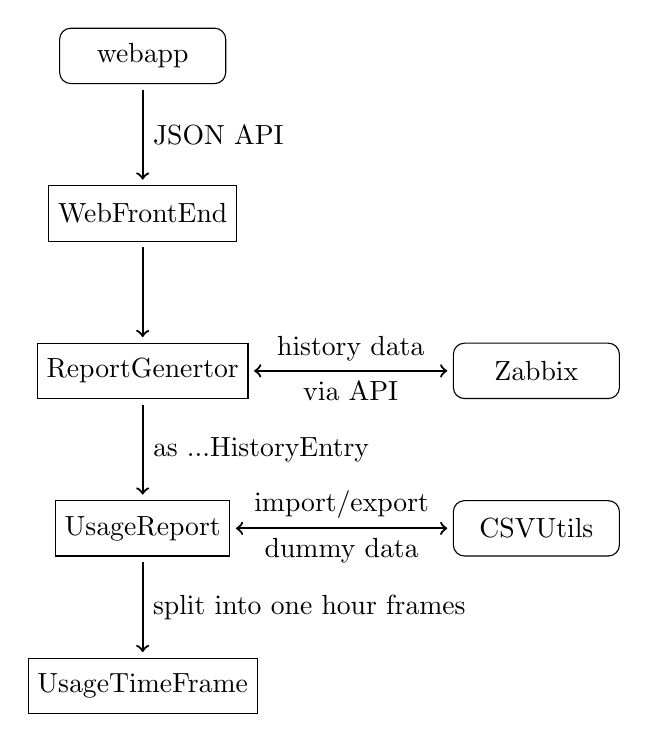
\begin{tikzpicture}
    \tikzset{
        external/.style = {
            rectangle, rounded corners, draw=black,
            minimum width=6em, minimum height=2em, text centered, node distance=5cm
        },
        internal/.style = {
            rectangle, draw=black,
            minimum width=6em, minimum height=2em, text centered, node distance=2cm
        },
        edge/.style = {
            ->, thick, shorten <= 2pt, shorten >= 2pt
        },
        dotted box/.style = {
            rectangle, draw = black, rounded corners, dashed, inner sep=3pt
        }
    };

	\node[internal] (generator) {ReportGenertor};
	\node[internal] (web) [above of = generator] {WebFrontEnd};
	\node[external, node distance = 2cm] (webapp) [above of = web] {webapp};
	\node[external] (zabbix) [right of = generator]  {Zabbix};
	\node[internal] (report) [below of = generator] {UsageReport};
	\node[external] (csv) [right of = report] {CSVUtils};
	\node[internal] (frame) [below of = report]{UsageTimeFrame};

	\draw[edge] (webapp) -- (web) node [midway, right] {JSON API};
	\draw[edge] (web) -- (generator);
	\draw[edge, <->] (generator) -- (zabbix)
		node [midway, above] {history data}
		node [midway, below] {via API};
	
	\draw[edge, <->] (report) -- (csv) 
		node [midway, above] {import/export} 
		node [midway, below] {dummy data};
	
	\draw[edge] (generator) -- (report)
		node [midway, right] {as ...HistoryEntry};
	\draw[edge] (report) -- (frame) 
		node [midway, right] {split into one hour frames};
\end{tikzpicture}

\section{}
Appendix two text goes here.


% use section* for acknowledgement
\section*{Acknowledgment}
The authors would like to thank...
\ifCLASSOPTIONcaptionsoff
  \newpage
\fi


\bibliography{bib/bibliography}{}
\bibliographystyle{plain}

\end{document}


